 %
% include the class file for GMP 2018  
%
\documentclass[submission]{gmp2018}
\usepackage{graphicx}
\usepackage{subfigure}

%%%%%%%%%%%%%%%%%%%%%%%%%%%%%%%%%%%%%%%%%%%%%%%%%%%%%%%%%%%%%%%%%%%%

\begin{document}

%
% put the title of your paper here
%
\title{Folding Cartons: Interactive Manipulation of Cartons from 2D Layouts}

%
% put your submission number here
% this number will appear instead of authors and affiliations if the class option "submission" is active
%
\SubNumber{1074}

%
% put the author names here
% use the second argument as a reference to the list of affiliations
% no authors and affiliations will appear if the class option "submission" is active
%
\author{Shuang Shan}{1}
\author{Yiting Ma}{1}
\author{Chengcheng Tang}{2}
\author{Xuejin Chen}{1}

%
% put the affiliations of the authors here
%
\affiliation{1}{University of Science and Technology of China}
\affiliation{2}{Stanford University}

%
% the rest is as usual
%
 

%\definecolor{red}{rgb}{1.0,0.0,0.0}
%\definecolor{blue}{rgb}{0.0,0.0,1.0}
\definecolor{purple}{rgb}{0.5,0.0,0.5}


\newcommand{\comments}[1]{}
\newcommand{\cxj}[1]{\textcolor{red}{(xuejin:#1)}}
\newcommand{\xjmd}[1]{\textcolor{purple}{#1}}
\newcommand{\vo}{\hat{\mathbf{v}}}
\newcommand{\vn}{\mathbf{v}}
\newcommand{\vset}{\mathbb{V}}


\newcommand{\reply}[1]{\textcolor{blue}{#1}}
%%%%%%%%%%%%%%%%%%%%%%%%%%%%%%%%%%%%%%%%%%%%%%%%%%%%%%%%%%%%%%%%%%%%

\maketitle

\begin{abstract}
Cartons are broadly used in packaging industry and our daily life. While most of traditional packages are axis-aligned cuboids, there is a recent trend of creating paper packages and cartons with more complicated geometry. In this work, we present an interactive system to manipulate 3D cartons from 2D layouts. Two key components, \emph{automatic folding} and \emph{suggestive editing}, make our system significantly easy to use. 
The automatic folding part automatically computes the 3D coordinates of vertexes in cartons based on simple observation. Then the suggestive editing part smartly provides a group of geometric constraints, such as vertex merging, merging propagation, and face pasting, for users to explore and manipulate 3D shapes.
Moreover, automatic updating of 2D layout is supported when the user edits the carton shape in 3D.  
\end{abstract}

\section{Introduction}

Cartons have been widely used in the packaging industry to organize, ship, and deliver various commodities, which include food, daily necessities, and electronic components. 
Beyond the very basic packaging shapes like cuboids, extremely elaborate packaging exists for certain specialty items, such as wedding candies or wine bottles. 
The popularity of such intricate designs has increased, not to mention the fact that they are environmental friendly due to their recycalbility and degradability~\cite{Mullineux:2010:CSC:1739328.1739673}.

Cartons are usually designed based on experience and trial-and-error.
Designers typically start a package design by generating 2D vector artwork; then, a 3D mockup is essential for designers and clients to see the real appearance~\cite{guide}. There are two ways to create a 3D mockup.
A digital mockup is a great, inexpensive way of showing how the design would appear in real life, plus it allows designers to repeatedly modify the layout.
%A digital mockup is a great way of showing how the design would appear with lower cost and is convenient for designers to modify the layout repeatedly. 
A physical mockup is also helpful when making sure the size is correct in order to make a final decision. 
%
Due to the low cost and efficiency of digital mockups, there have been many software packages developed to help designers improve their design efficiency and productivity.
%
For example, the commercial software named STUDIO~\cite{STUDIO} generates 3D models by manually assigning angles to folding edges. 
By using models, users can turn their ideas into beautiful 3D images.
Moreover, it is non-trivial for non-expert users to figure out how to fold a complex carton using only a 2D crease pattern. A digital simulation system would provide valuable references to inspire creativity~\cite{Thiel1998,Kishi:1998:OFP:786112.786279,Nimnual2007Virtual}. 
However, the existing softwares still requires extensive manual skill to design cartons.
%Researchers have also studied in obtaining 2D layouts from unfolding 3D objects for decades. However, the unfolded layouts are fragile in some parts which are not suitable for fabrication~\cite{Tai2004Unfolding} and sometimes are not feasible to fold.
In order to create a virtual 3D model and explore diverse layouts, our idea is to fold the existing layout directly into a 3D model, and reach a variety of layouts by manipulating the corresponding model.


It is nontrivial to mathematically formulate the problem of model construction using only a planar layout, because the information extracted from the 2D pattern, such as edge length and vertex degree, may cause ambiguities on account of repeated edges and vertexes. 
Moreover, Biedl et al.~\cite{Biedl:2005:NFP:1090462.1646553} proved that given a polygon and a set of creases, it is NP-hard to know whether a polyhedron can be obtained by folding along the creases, which can also illustrate the difficulty of our problem.

\begin{figure}
	\centering
	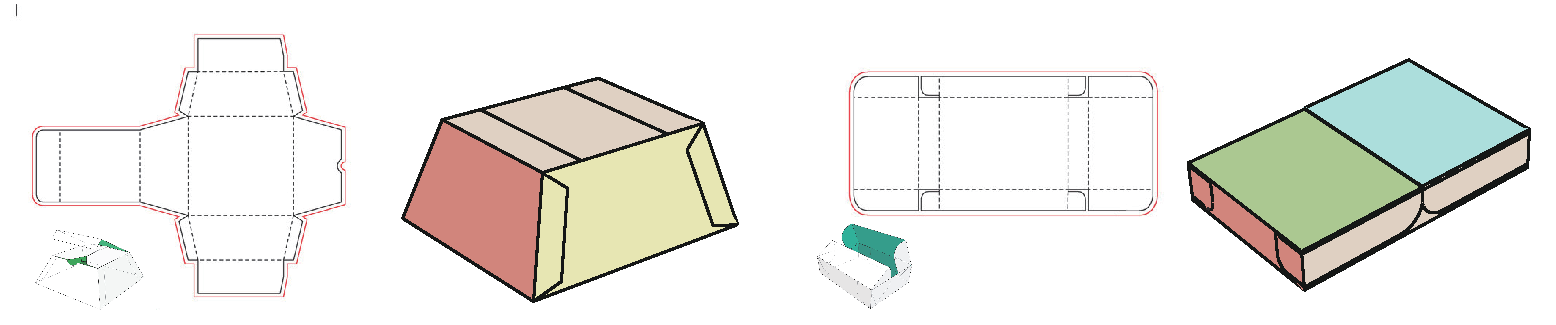
\includegraphics[width=0.9\textwidth]{images/artist}
	\caption{Two cartons and artist-designed layouts. The corresponding 3D models are folded according to our system.}
	\label{fig:artist}
\end{figure}

 
 
In order to solve the folding cartons using 2D layouts as our only input, we present an optimization method when given a set of shape constraints.
Moreover, an interactive design and exploration framework is proposed to allow users to visualize planar layouts and corresponding models in a 3D view and freely edit the models. 
The original layout can be corrected and explored by optimization. Figure~\ref{fig:artist} shows our folding results based on a series of 2D layouts designed by artists. 

The contributions of this paper includes the following:

(1) An interactive and explorative system to manipulate the shapes of 3D cartons. Our system creates corresponding models using rough initializations and user interactions. Imprecise layouts can be modified with a geometric optimization. Users may easily edit these 3D models in order to explore alternative deformed layouts
%3D model by a rough initialization and user interactions, and modifies imprecise layouts by a geometric optimization. Users are allowed to edit the 3D model to explore deformed layouts automatically.

(2) A collection of shape constraints, which are represented through a set of points, are used to implement shape optimization. Based on observations of existing cartons, constraints are summarized by including panel rigidity and coplanarity to maintain the integrity of the cartons' shapes. 
In addition, computer-aided detection, like vertex merging and panel pasting, is introduced to offer suggestions to users. 
\section{Related Work}\label{sec:relatedwork}
\subsection{Folding problem}

Origami folding, producing a 3D shape from a single piece of planar sheet, has been widely studied for decades. Earlier techniques focus on the simulation of the folding process given the 2D crease pattern and its corresponding configuration of fold angles~\cite{Thiel1998,Kishi:1998:OFP:786112.786279,Nimnual2007Virtual}. Typically, these simulation systems require the folding order and angles of the creases in the 2D pattern. 
%
While a 2D crease pattern with mountain or valley type is given, a continuous process can be simulated for designing transformable and deployable structures~\cite{tachi2009simulation,tachigeometric}.
%
Above simulation systems primarily apply to paper origami with zero-thickness. Recently, many techniques~\cite{tachi2011rigid,chen2015origami,2016arXiv160105747K} were proposed to develop the kinetic synthesis for thick panels that can be folded identically to zero-thickness origami in mechanical engineering.
%
These simulation systems are limited to the flat-foldable rigid origami with known mountain or valley crease types. In comparison, our system only takes the 2D crease pattern as input without knowing the folding angles of the creases. 

 
There are also some methods to solve related problems of carton folding. 
Song et al.~\cite{Song:2000:MPA:892954} modeled foldable objects as tree-like multilink objects and used the probabilistic roadmap methods~\cite{Kavraki:1994:PRP:891758} to find a sequence of motions to transform one configuration of a foldable object into another configuration. 
Mullineux et al.~\cite{Mullineux:2010:CSC:1739328.1739673} provided a simulation framework for carton erection considering geometric constraints for assembly.
Both of these two methods require the target 3D state given as a premise, while our work aims to recover the 3D configuration of the folded carton from a 2D layout.

\reply{ 
 Compared with straight creases in above approaches, curved folding, involving curved folds in the crease pattern, has also drawn attentions in computer graphics.  %
 Kilian et al.~\cite{Kilian:2008:CF:1360612.1360674} presented an optimization-based framework to reconstruct a 2D development from a reference 3D surface.
 %
 Solomon et al.~\cite{Solomon:2012:FDS:2346796.2346817} introduced a discrete paradigm to model developable surfaces based on 2D configurations, where the crease pattern and the corresponding crease angles are pre-defined.
% provided a subdivision based modeling scheme involving curved paper structure with folding angles on creases as input. 
Recently, Kilian et al.~\cite{Kilian:2017:SAC:3087678.3015460} designed practical mechanisms to fabricate a curved folded surfaces simply by pulling a network of strings. 
%the deformation of curved folded surfaces after the folding motion actuated by pulling a network of string. 
%
By contrast, we focus on an inverse problem of recovering the 3D shape from a 2D planar pattern without knowing any 3D information.
}

%The extra 3D information is represented as target 3D objects, folding angles or external forces above.
 



\comments{
Folding two-dimensional pattern into three-dimensional objects has been studied in various fields, such as rigid origami folding, curved folding and carton folding. Despite the 2D pattern as an input, all of these problems need extra 3D information or interactions, while this paper chooses the 2D layout as only input.

Rigid origami folding is similar to our problem, while the folding motion is mostly computed based on the given angle of creases, and consider the geometry of origami in kinetic motion~\cite{tachi2009simulation,tachigeometric}. The thickness problem of origami is also a direction of origami related research these years, and its goal is to simulate the folding behaviour exactly the same to when folding paper with zero thickness by designing different connecting structures between panels~\cite{chen2015origami,2016arXiv160105747K,tachi2011rigid}. Thick origami folding problem also has a target configuration to approximate.



There are also some methods to solve related problems of carton folding. 
Song et al.~\cite{Song:2000:MPA:892954} modeled foldable objects as tree like multilink objects and used PRMs~(probabilistic roadmap methods~\cite{Kavraki:1994:PRP:891758}) to find a sequence of motions to transform one configuration of a foldable object into another configuration. 
Mullineux et al.~\cite{Mullineux:2010:CSC:1739328.1739673} provided a simulation framework of the carton during erection using a constraint-based approach. Both these work required the target state as a premise, while our work aims to generate the target configuration.

Folding 2D layouts with interactive tools visualizes the folding behaviour of a single piece of paper. Thiel~\cite{Thiel1998} provided a virtual origami system including the user interface to model folded paper and show animations of folding process. Kishi et al.~\cite{Kishi:1998:OFP:786112.786279} allowed users to create and edit the origami properties over the Web. Nimnual et al.~\cite{Nimnual2007Virtual} presented an application for package folding practices in a virtual space. Although these applications can model folded paper well, they need given parameters to construct the model, or their final goal is flat folding which can also be seen as a premier to the problem.

In addition, the above works cannot edit corresponding 3D model and optimize its layout in turn, which is one of the advantages of our system.
}
 

\subsection{3D reconstruction of line drawings}
\reply{Although having the same goal of constructing 3D models from 2D layouts including vertexes and edges, there is a one-to-one correspondence between the vertexes in the 2D line drawing and 3D model, while our problem recovers many-to-one correspondences and the 3D construction process is different.} 

A line drawing is defined as a 2D projection of a object containing its vertexes and edges. 3D interpretation of line drawings have been studied for a long time. 
%The main problem is in object reconstruction given its projection on two-dimensional planes. 
Some researchers treat this task as an optimization problem. 
Marill~\cite{Marill:1991:EHI:113057.113061} first proposed the principle of minimizing the standard deviation (MSDA) of angles to emulate the interpretation of line drawings as 3D objects. 
%
This new criterion was used by many other researchers soon after. 
Leclerc et al.~\cite{Leclerc1992An} combined MSDA with the deviation from planarity as objective terms. 
Cao et al.~\cite{Cao:2005:ORS:1097114.1097658} added a symmetry metric of 3D objects to get more complicated results. 
Some other researchers tried to solve this problem from the point of view of information theory.
%
Marill~\cite{Marill1992Why} minimized the description length of objects based on the idea that humans usually pick the simplest one from infinite possibilities when they see the line drawing. 
Shoji et al.~\cite{Shoji20013} minimized the entropy of the angle distribution between line segments by a genetic algorithm. 
Later, the strategy of splitting and merging was used to reconstruct line drawings of complex 3D objects~\cite{10.1109/TPAMI.2010.49,10.1109/CVPR.2014.94}.   
		 
Different from line drawings, our input is the expanded structural layouts in 2D planes of 3D carton objects.
The 3D carton model is constructed based on the folding procedure instead of the mathematical projection from 3D to 2D.

\subsection{Geometrical shape optimization}
%\reply{The basic idea of our paper is  shape optimization under a set of simple constraints.}
In geometrical shape processing, many algorithms have been proposed to enforce shape constraints, and have been successfully used in interactive tools and physical simulation~\cite{Botsch:2006:PCP:1281957.1281959,Igarashi:2005:ASM:1186822.1073323}. 
Bouaziz et al.~\cite{Bouaziz:2012:SSD:2346796.2346802} unified a large variety of geometric constraints into one optimization framework, and provided a simple and robust implementation. 
Poranne et al.~\cite{Poranne2013Interactive} described an interactive method to manipulate and optimize polyhedral meshes under constraints with a linear-time algorithm. 
%
Tang et al.~\cite{Tang:2014:FPM:2601097.2601213} solved constrained equations by Newton-type method in a fast way, and provided an interactive system to model meshes constrained by equalities and inequalities. 
Deng et al.~\cite{Deng2015} developed an interactive tool to explore architectural design with shape constraints, and provided an optimization method to enforce hard constraints and soft constraints at the same time. 

\xjmd{The studies mentioned above focus on optimizing existing 3D shapes with geometric constraints, and propose different optimization solutions.
%
2D layouts are not involved in their problems.
In contrast, our goal is to recover the structure and topology from an expanded layout to form a 3D carton model.
The geometric constraints are automatically detected and presented for users to explore during the folding process. }
%correspondence and our constraints do not need satisfy properties like fairness. 
%In our paper, we implement the shape optimization by the method introduced in \cite{Bouaziz:2012:SSD:2346796.2346802} for its robustness and simplicity.




\section{Overview}\label{sec:overview}


Figure~\ref{fig:overview} shows the overview of our algorithm. 
The input 2D layout of a carton consists of a set of cutting edges (solid lines) and folding edges (dashed lines).
%
Given the 2D layout, an undirected graph is built, and a set of polygonal panels are extracted by finding the minimum cycles in the graph, as Figure~\ref{fig:overview}(b) shows. 
Therefore, the 2D layout can be represented by a polymesh $\mathcal{L}=(V,E,P)$, where $V$ is the set of vertexes, $E$ is the set of all edges, and $P$ is the set of panels. 
The edge set $E=E_c\cup E_f$, where $E_c$ is the set of cutting edges, and $E_f$ is the set of folding edges.
%
To build a 3D carton model $\mathcal{M}=(V, E, P)$ from the 2D layout $\mathcal{L}$, which share the same topology, we compute the 3D coordinates of all of the vertexes in $V$. 
%

However, it is not intuitive to analytically define the desired final 3D shape from a 2D layout. 
One possible alternative is to detect all the possible geometric constraints, such as vertex merging, panel parallelism, orthogonality between adjacent panels, and then integrate all these possible constraints together to form a large equation system. 
The challenge is that these local constraints can not adequately describe complicated and creative designs. 
Moreover, there are many ambiguities when detecting these constraints in a 2D layout, such as edges and panels that exist within the same shape. 
%
We propose a two-step algorithm based on the observation that humans usually fold edges at a right angle in order to obtain a rough shape, and then they merge the vertexes or edges to create a stable 3D carton.
% Our algorithm consists of two steps. 
First, an initial 3D model (Figure~\ref{fig:overview}(c)) is constructed based on a specific angle along each folding edge, as described in Sec.~\ref{sec:initialization}.
The user can then manipulate and explore the various 3D shapes of the carton based on a series of suggested operations provided by our system. 
%
The final model is shown in Figure~\ref{fig:overview}(e).
The details of each step are introduced in the following sections. 
 
\begin{figure}
	\centering
	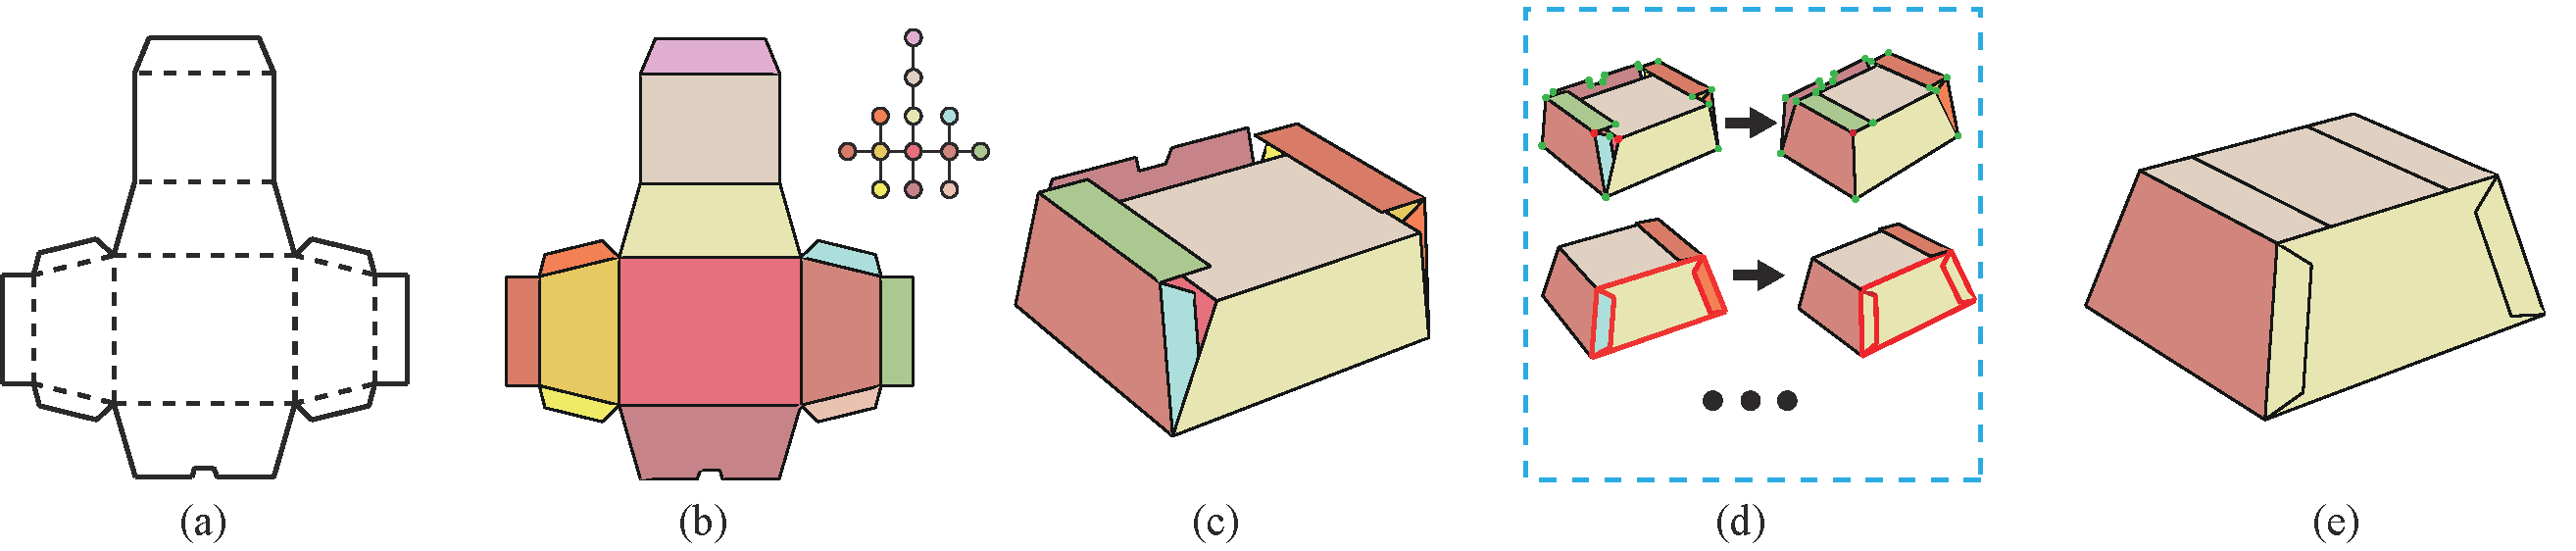
\includegraphics[width=0.9\textwidth]{images/overview}
	\caption{Given a 2D layout (a), we first extract its 2D mesh (b) with different panels in different colors. By providing each folding edge with the same angle, which is $\pi/2$, an initial 3D model can be constructed~(c). The final carton model (e) is built by a shape optimization technique based on a series of suggested geometrical constraints (d).}
	\label{fig:overview}
\end{figure} 
 



\subsection{Shape Initialization}\label{sec:initialization}

\cxj{re-write this section. Describe clearly about the parameters, the objective, and methods. }

In this section we explain the reason why using a specific angle to each fold edge, and constructing our initialized model. The basic ideal is to interpret the folded state of a box as a series of rotation angles along each edge, and by setting specific value of angles which is $\pi/2$, we can have a rough model to assist the later optimization.
		
Observed from existing data in the Internet, most of the traditional cartons are cuboid, as the examples shown in Figure~\ref{fig:realdata} (a) and (b), they are used to put in files or delivering daily supplies. Although there is a recent trend to design more complicated layouts to attract consumers Figure~\ref{fig:realdata} (c), the shape of these unusual cartons is similar to orthogonality boxes as their functions are still packaging commodity. Based on this observation, we set $\pi/2$ as the value of rotation angle to each fold edge, and have the initialized model as Figure~\ref{fig:initial}.

As shown in Figure~\ref{fig:initial} (a), the traditional cartons as cuboid boxes can reach an ideal state, while the novel designs need a little refinement like the four examples in Figure~\ref{fig:initial} (b). Take the hexagonal box as an example, users only need to assign six paste faces into corresponding surface, the model of a feasible carton will be generated. As a result, we interactively allow users to add these constrains into our system and optimize to a desired model.

\begin{figure}
	\centering
	\includegraphics[width=0.9\textwidth]{images/realdata.jpg}
	\caption{Two traditional cartons (a), (b) and one unusual carton (c) with their corresponding layouts.}
	\label{fig:realdata}
\end{figure}

\begin{figure}
	\centering
	\includegraphics[width=0.9\textwidth]{images/initial.jpg}
	\caption{Eight different initialization results. Four initial cartons shown in the second column of (a) can reach the ideal state, the other four cartons need further refine (b).}
	\label{fig:initial}
\end{figure}

%%%%%%%%%%%%%%%%%%%%%%%%%%%%%%%%%%%%%%%%%%%%%%%%%%%%%%%%%%%%%%%%%%%%%

%\section{Algorithm}\label{sec:optimization}



\subsection{Shape Refinement}\label{sec:refinement}

%there is still a need to refine the results that have not folded into pleasing results. 
Though not perfect, the initial 3D shape provides a good start point for generating the final carton model. 
%
To further refine the 3D shape, the 3D coordinates of all the vertexes are then refined based on a set of shape constraints, such as vertex merging, panel pasting, and so on.
%
%the main idea is to prescribe the shape constraints by a set of vertexes of the polymesh. 
%Moreover, with the extra information acquired from user interaction, we can finally construct the desired 3D realization.
In this step, the coordinate of vertexes are chosen as our objective instead of angles on folding edges, mainly because that the geometric constraints in 3D shapes can be more simply and intuitively represented by 3D vertex coordinates.
% and we can implement the algorithm introduced by Bouaziz et al. easily~\cite{Bouaziz:2012:SSD:2346796.2346802}.


%\subsection{Aided Detection}

%While the initial 3D model with simple angle folding provides a rough idea about the carton shape, 
A suggestive interface is provided to users for efficiently exploring better carton shapes, as described later in Sec.~\ref{sec:interaction}. 
%
Once the user selects a suggested shape refinement operation, we optimize the 3D shape based on a series of geometric constraints.
%We now introduce the constrains used in our construction method:
Given the current mesh whose vertex positions are defined as $\{\vo_i\}^{N}_{i=1}$, a new mesh with the same topology but new vertex positions $\{\vn_i\}^{N}_{i=1}$ will be computed according to the specified shape constraints.
%
The geometric constraints can be classified into two groups, shape rigidity constraints and shape modification constraints.
% 
First, to keep the rigidity of each panel, the constraints including panel rigidity and coplanarity, corresponding to the similarity constraint and plane constraints described in \cite{Bouaziz:2012:SSD:2346796.2346802}. 
%
Second, once vertexes or panels are confirmed to be merged to modify the rough shape, more constraints are added. 
%
Each constraint is defined as following.  

\comments{
\paragraph{Edge length constraint.} 
For each edge in $\{e_j\}_{j=1...M}$, its length should be preserved when refine the carton shape.
Hence, its two endpoints $\mathbf{v}_{js}$ and end point $\mathbf{v}_{jt}$ should satisfy 
\begin{equation}
||\mathbf{v}_{js} - \mathbf{v}_{jt}||^2 = ||\mathbf{\hat{v}}_{js} - \mathbf{\hat{v}}_{jt}||^2.
\label{equ:edge}
\end{equation}
%to ensure that the length of each edge stays the same.
}


\paragraph{Panel rigidity.} 
Each panel keeps its shape unchanged during folding. This constraint is defined by keeping the length of each line connecting any pair of points $\mathbf{v}_{a}, \mathbf{v}_{b}$ on the panel the same.
\begin{equation}
||\mathbf{v}_{a} - \mathbf{v}_{b}||^2 - ||\hat{\mathbf{v}}_{a} - \hat{\mathbf{v}}_{b}||^2 = 0.
\label{equ:plane}
\end{equation}




\paragraph{Coplanarity.} {For each panel $P_{k}$, the coplanarity constraint specifies that all vertexes in this panel should always lie on a plane. 
We can compute the sorted eigenvectors $\mathbf{U} = [\mathbf{e}_1, \mathbf{e}_2, \mathbf{e}_3]$ of the $ 3 \times 3$ covariance matrix $\mathbf{C}^T\mathbf{C}$ where $\mathbf{C} = \{\mathbf{v}_{kj}\}_{j=1}^{N_k}$, $\mathbf{v}_{kj}$ is the $j^{th}$ vertex among $N_k$ vertexes in the panel. By removing the last column of $\mathbf{U}$, we can implement plane projection as \cite{Bouaziz:2012:SSD:2346796.2346802} described.


If a set of shape modification operations, such as vertex merging and panel pasting, are selected, more constraints are added to optimize the vertex positions. 
%
%and one of the interaction is to choose the right given suggestion including points needed to be merged together. As for the point information, the constrains can be written like:

\begin{figure}
	\centering
	\subfigure[Vertex merging]{
		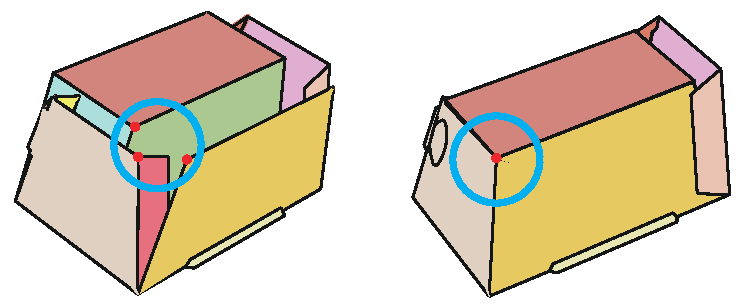
\includegraphics[width=0.45\columnwidth]{images/vertexmerging}
		\label{fig:vertexmergingBeforeAfter}
	}
	\hfill
	\subfigure[Panel pasting]{
		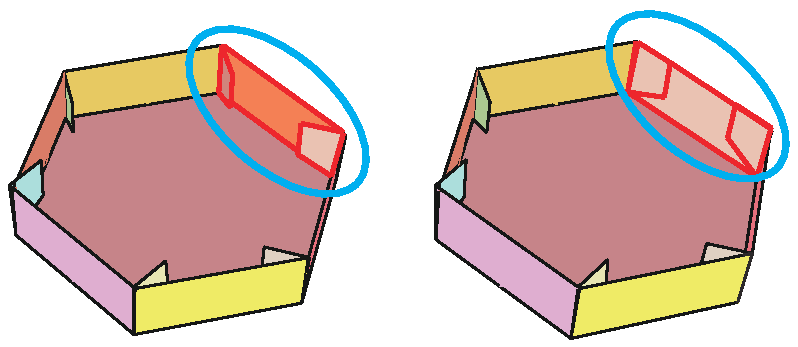
\includegraphics[width=0.45\columnwidth]{images/facemerging}
		\label{fig:facemergingBeforeAfter}
	}
	\caption{3D shape refinement based on merging vertexes (a), or pasting panels (b). The locations where the 3D shape changes are highlighted in blue.  }
	\label{fig:shaperefinement}
\end{figure}

\paragraph{Merging vertexes.} 
For any two vertexes $\mathbf{v}_p$ and $\mathbf{v}_q$ that are selected to be merged as the same vertex, we have 
\begin{equation}
\mathbf{v}_p - \mathbf{v}_q = \mathbf{0}.
\label{equ:point}
\end{equation}
%if these two points $\mathbf{v}_p$, $\mathbf{v}_q$ need to be moved into the same place. 

\paragraph{Panel pasting.}
%If a smaller face $f_a$ is snapped to a larger face $f_b$, for each vertex $\vn_i$ in the face $f_b$, we have
%\begin{equation} \label{eq:face-paste}
%\vn_i \cdot \mathbf{n}_a = 0,
%\end{equation}
%where $\mathbf{n}_a$ is the normal of the face $f_a$.
If two panels $P_a$ and $P_b$ need to snap together, all the vertexes of these two panels should satisfy the same coplanarity constraint. 


%When the above constrains still lead to an ill-posed problem, soft constraints will be added to keep the original positions of the vertices that are not relative to the shape modification. 

\reply{Typically only a few shape modification operations are selected at each time, the above constraints form an under-constrained system to solve the new vertex coordinates. In order to find a feasible solution for the constrained problem,} soft constraints will be added to keep the original positions of the vertexes that are not relative to the selected shape modification.

\paragraph{Irrelevant vertexes.} For the vertexes not in the same panel with any vertex for merging or panel pasting, they should stay at their original locations. 
We add these soft constraints by adding a small weight $w$, which is set to 0.001 in our experiments to the following equation. 
\begin{equation}
w(\mathbf{v}_i - \mathbf{\hat{v}}_i) = \mathbf{0}.
\label{equ:irrelevant}
\end{equation}

\reply{Bouaziz et al.~\cite{Bouaziz:2012:SSD:2346796.2346802} proposed an efficient optimization method that could combines all these shape constraints together. We directly use their C++ library ShapeOp to solve our shape optimization problem once a shape modification operation is performed.}
Figure~\ref{fig:shaperefinement} shows two examples of shape refinement by merging three vertexes and pasting three panels respectively. 

\comments{
Combining the above constraints, the new vertex locations can be solved by minimizing the proximity function based on projection operators~\cite{Bouaziz:2012:SSD:2346796.2346802}. 
%
\reply{For a single point $\mathbf{v}$, the proximity function is defined as
\begin{equation}
\phi(\mathbf{v}) = \sum_{i=1}^{m}\omega_i{d_i(\mathbf{v})}^{2},
\label{equ:function}
\end{equation}
where $\omega_i$ are non-negative weights, and $d_i$ is the distance between the point $\mathbf{v}$ and its projection onto the constraint set, $m$ is the number of constraints. For all the vertexes $\mathbf{V} = \{\mathbf{v}_i\}_{i=1\dots n}$, the shape proximity function is formulated as
\begin{equation}
\phi(\mathbf{V}) = \sum_{i=1}^{m}\omega_i||\mathbf{N}_i\mathbf{V}_i-P_i(\mathbf{N}_i\mathbf{V}_i)||_2^2,
\label{equ:function2}
\end{equation}
where $\omega_i$ are weights and $P_i(\cdot)$ is the projection onto the constraint. The matrix $\mathbf{N}_i$ is used to center the vertexes at their mean.
}
}
%


\section{User Interaction}\label{sec:interaction}
After initializing the flat mesh, we need to refine the model to final state through the shape constrain proposed and the information acquired from user interaction. The system provides a set of operations to assist users construct the optimized model, such as selecting points that need to be merged together. Moreover, the system can automatically detect the points that need to be located in one place and provide suggestions to allow users click the right option.

Figure~\ref{fig:interface} illustrates two operations that the system provides, the first one is selecting points need to be merged by users and the second is select the right option from results by auto-detection.   

\begin{figure}
	\centering
	\includegraphics[width=0.9\textwidth]{images/UIdetail.jpg}
	\caption{two operations that the system provides}
	\label{fig:interface}
\end{figure}
\section{Results and Discussion}\label{sec:result}
{\color{red}{SS: Any need to list the number of steps we take to generate final model?}}

The step of shape optimization in our paper can be best demonstrated on the model~\ref{fig:result}, through initialization, we can have a rough concept of the final model, and by user interaction including selecting vertices merged and faces in the same plane, we can finally generate a pleasing model from a given structural layout.

We show a number of 3D models generated by our system Figure~\ref{fig:more}, and most of the cases can have an ideal result after initialization because of the cuboid shape as Figure~\ref{fig:more} (a). Through interaction, users can folding more complicated cartons to ideal shapes as Figure~\ref{fig:more} (b).

However, the initialization will not generate a pleasing result on some complicated cases, and leads to the difficult interaction to get the final model. As for Figure~\ref{fig:limitation}, to have a better corresponding model, users need to take at least ten steps to get to Figure~\ref{fig:limitation}(c). 


\begin{figure}
	\centering
	\includegraphics[width=0.9\textwidth]{images/result.jpg}
	\caption{Structural layout (a) is used to generate flat polymesh (b), and then initialize to a rough model (c), after merge the three vertices in red circles (c) and the two vertices circled red (d), the model is almost closed with two paste faces in red and pink outside the carton (e), finally through selecting these faces are in the same plane of the yellow face as surface, we can have the final model (f).}
	\label{fig:result}
\end{figure}

\begin{figure}
	\centering
	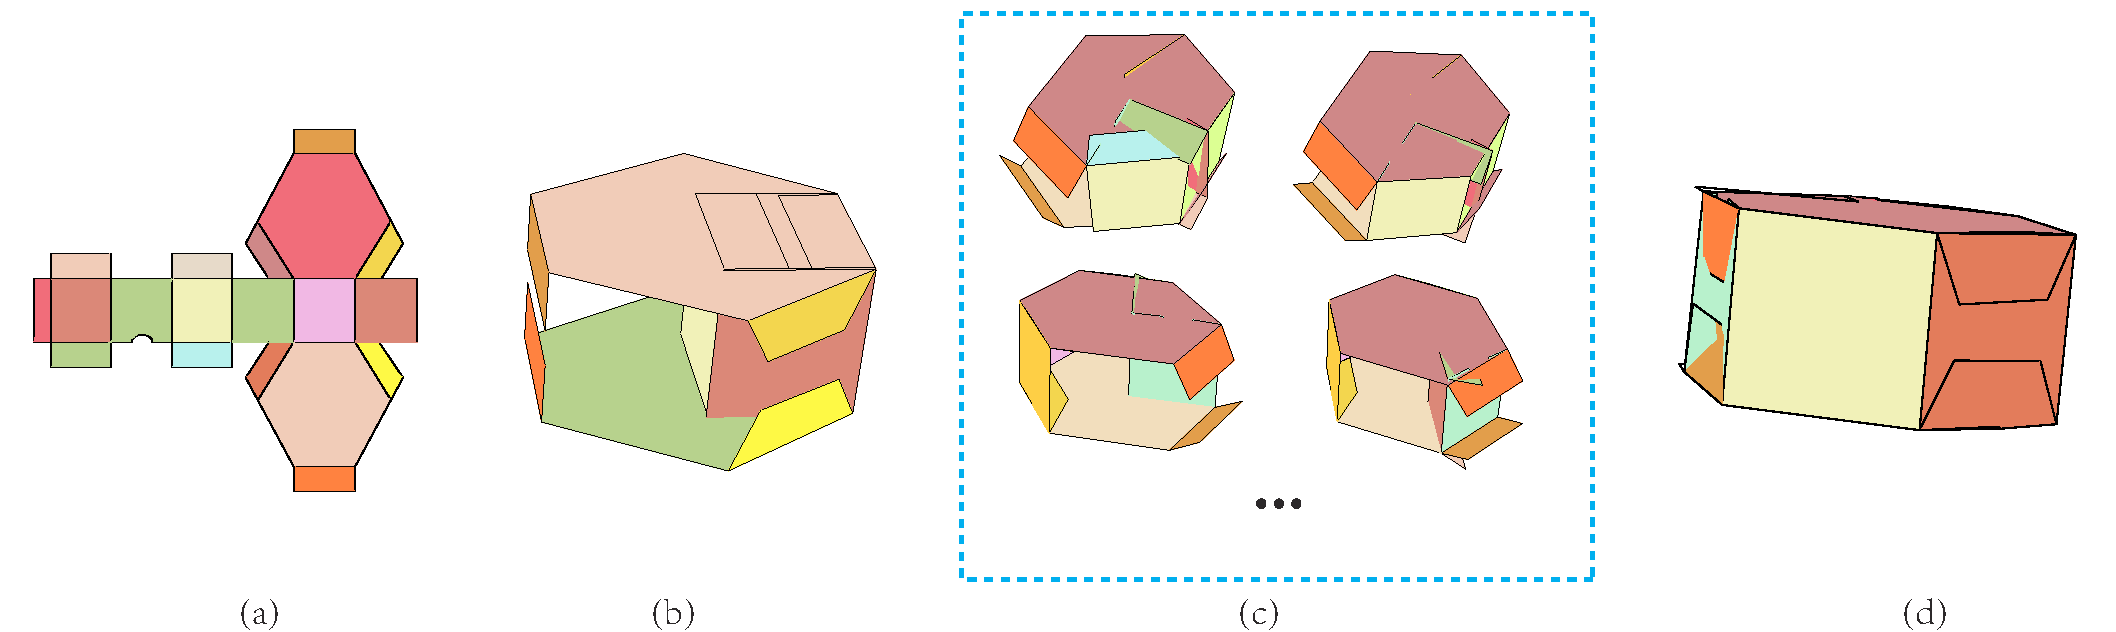
\includegraphics[width=0.9\textwidth]{images/limitation.jpg}
	\caption{Given a layout as (a), our system can generate an initialized result as (b), and through at least ten steps including select vertices need to be the same place and faces need to be coplane , users can get the final model as (c).}
	\label{fig:limitation}
\end{figure}

\begin{figure}
	\centering
	\includegraphics[width=0.9\textwidth]{images/more.jpg}
	\caption{More results, part of cartons can be initialized without refining (a), and with interaction, users can manipulate more complicated cartons (b). The first and second column in (a) and (b) are the flat mesh and initialization result of cartons, and the last column in (b) shows the model after interaction.}
	\label{fig:more}
\end{figure}

%%%%%%%%%%%%%%%%%%%%%%%%%%%%%%%%%%%%%%%%%%%%%%%%%%%%%%%%%%%%%%%%%%%%%

\section{Conclusion and Future Work}\label{sec:conclusion}
In this paper, we present an interactive modeling system to construct a 3D carton model from a 2D expanded layout. 
Based on the automatically folded rough model, a series of shape refinement suggestions are provided for smartly optimizing and editing the carton model, which assists users on producing the desired model efficiently and productively. 
%
Our current system could be further improved in many directions. 
More intelligent editing tools can be implemented. For example, when the user moves a vertex, the vertex translation can be propagated to other symmetric vertexes.
We also would like to improve our automatic folding part with a more comprehensive optimization formulation considering both shape closure and stability. 
%
Moreover, it is desired by designers to support appearance editing in our system.
%

%%%%%%%%%%%%%%%%%%%%%%%%%%%%%%%%%%%%%%%%%%%%%%%%%%%%%%%%%%%%%%%%%%%%

\bibliographystyle{abbrv}
\bibliography{ref}

\end{document}
